\documentclass{article}
\usepackage[a4paper, total={6.5in, 10in},top=2cm]{geometry}
\usepackage[bottom,hang]{footmisc}
\usepackage{amsmath}
\usepackage{amsfonts}
\usepackage{graphicx}
\usepackage[plain]{algorithm}
\usepackage{enumitem}
\usepackage{algpseudocode}
\usepackage{ragged2e}
\usepackage[usenames,dvipsnames]{color}
\usepackage{xcolor}
\usepackage[most]{tcolorbox}
\usepackage{hyperref}
\usepackage{dirtree}
\usepackage{textpos}
\usepackage{marginnote}
%\usepackage[newfloat]{minted}
\usepackage{caption}
\usepackage{xepersian}

%\SetupFloatingEnvironment{listing}{name={کد}}
\setlength{\footnotemargin}{2mm}
\setlist{itemsep=1pt}

\graphicspath{{./images/}}
\DeclareGraphicsExtensions{.pdf,.jpeg,.jpg}

\delimitershortfall=-1pt
\hypersetup{
	colorlinks=true,
	linkcolor=blue,
	filecolor=,
	urlcolor=blue,
}

\settextfont[Scale=1.1]{XB Kayhan}
\setlatintextfont[Scale=1.1]{Times New Roman}
\DefaultMathsDigits
\setlength{\skip\footins}{1.2pc plus 5pt}

%\setlist[enumerate,1]{label={(\arabic*)}}

\definecolor{light-gray}{gray}{0.95}
\definecolor{lighter-blue}{HTML}{EDF1F4}
\definecolor{light-blue}{HTML}{12558E}
\definecolor{light-orange}{HTML}{F4F0ED}
%EDE4DD

\linespread{1.5}

\setlength\parindent{0pt}

\newenvironment{answer}{}{\\[.3ex]}
\newenvironment{question}[1]{\textbf{#1.} }{}
\tcolorboxenvironment{question}{enhanced,size=fbox,colback=lighter-blue,boxrule=0pt,sharp corners}

\newenvironment{qitem}[1]{%
	\begin{enumerate}\item[(#1)]}{\end{enumerate}}
\tcolorboxenvironment{qitem}{enhanced,size=fbox,colback=light-orange,boxrule=0pt,sharp corners}

\newtcbox{\code}{on line,fontupper=\ttfamily,size=fbox,colback=light-gray,boxrule=0pt,sharp corners}

\newtcolorbox{titlebox}{enhanced,size=normal,colback=light-gray,colframe=black,sharp corners,shadow={-1mm}{-1mm}{0mm}{black},boxrule=0.6pt,boxsep=2mm}
\newtcolorbox{hints}[1][]{colback=blue!10!white,colframe=blue!50!black,title=#1,fonttitle=\bfseries\large}

%\tcbset{highlight math style={enhanced jigsaw,size=fbox,colback=light-gray,boxrule=0pt,sharp corners}}

\newcommand{\Institute}{دانشکده مهندسی کامپیوتر}
\newcommand{\Title}{تمرین اول}
\newcommand{\DueDate}{۱۴۰۰/۰۱/۱۴}
\newcommand{\Class}{آزمون نرم‌افزار}
\newcommand{\Instructor}{دکتر حسن میریان}
\newcommand{\ClassCode}{40828}

\definecolor{pblue}{rgb}{0.13,0.13,1}
\definecolor{pgreen}{rgb}{0,0.5,0}
\definecolor{pred}{rgb}{0.9,0,0}
\definecolor{pgrey}{rgb}{0.46,0.45,0.48}
\definecolor{customblue}{RGB}{235,241,245}
%
%\newmintedfile[Javacode]{java}{
%	fontfamily=tt,
%	fontsize=\footnotesize,
%	bgcolor=customblue,
%	formatcom=\setLTR,
%	linenos=true,
%	numberblanklines=true,
%	numbersep=5pt,
%	escapeinside=||,
%	gobble=0,
%	%frame=leftline,
%	frame=single,
%	framerule=0.4pt,
%	framesep=3mm,
%	funcnamehighlighting=true,
%	tabsize=3,
%	obeytabs=false,
%	mathescape=false,
%	samepage=false, %with this setting you can force the list to appear on the same page
%	showspaces=false,
%	showtabs =false,
%	texcl=false,
%	breaklines=true,
%	baselinestretch=1.1
%}

\begin{document}
	\begin{textblock*}{\textwidth}(0pt,-1.5cm)
		\centering \small
		بسمه تعالی
	\end{textblock*}
	\begin{minipage}[c]{0.7\textwidth}
		\flushright
		{\Large\bfseries{\Class} (\ClassCode)}\\
		{\small استاد: \Instructor}
	\end{minipage}
	\hfill
	\begin{minipage}[c]{0.17\textwidth}
		\centering
		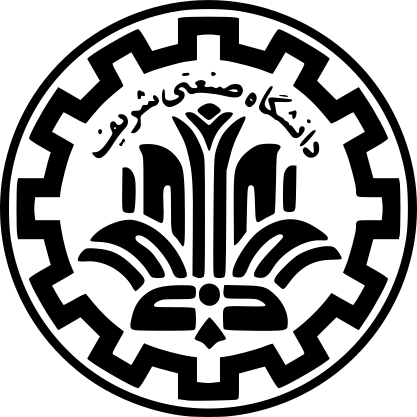
\includegraphics[width=.6\textwidth]{sharif-logo}\\[-5pt]
		{\scriptsize \Institute}
	\end{minipage}
	\vspace{2ex}
	\begin{titlebox}
		{\Large{\textbf{\Title}}}\hfill
		\parbox{.4\textwidth}{%
			\vspace{-1.3ex}
			\flushleft
			\small
امیرحسین کارگران خوزانی {\footnotesize (۹۹۲۰۱۱۱۹)}\\
سید سجاد میرزابابایی {\footnotesize (۹۹۲۱۰۱۴۲)}\\
رامتین باقری {\footnotesize (۹۹۳۰۱۹۳۸)}
		}
	\end{titlebox}
% ~~~~~~~~~~~~~~~~~~~~~~~~~~~~~~~~~~~~~~~~~~~
\subsection*{بخش نظری}
\begin{question}{1}
در این بخش باید یک برنامه تبدیل اعداد رومی به اعداد دهدهی را مورد بررسی قرار دهید. این برنامه به زبان برنامه‌نویسی جاوا نوشته شده است.
\end{question}
\begin{qitem}{a}
خطا یا خطاهای برنامه در کدام قسمت هستند؟ اصلاح‌شده آنها را بنویسید.
\end{qitem}
\begin{answer}
خروجی مورد انتظار این تابع برای ورودی \code{II} مقدار \code{2} خواهد بود؛ اما پس از اجرای تابع با ورودی مذکور، مقدار \code{0} نتیجه می‌شود. این مشکل از آنجا سرچشمه می‌گیرد که افزودن عدد جدید به اعداد قبلی \textbf{تنها} در صورتی انجام می‌شود که شرط \code{next > currentNumber} برقرار باشد، با این حال نیاز است تا برابری این دو متغیر نیز برای افزودن عدد لحاظ شود.
چرا که در غیر این صورت در اعدادی مانند \code{II} که یک کاراکتر پشت‌سرهم تکرار شده است خطا ظاهر می‌شود.
با تغییر در خط ۲۳ و اضافه کردن حالت برابری دو متغیر، مشکل حل خواهد شد. نسخه اصلاح‌شده برنامه در \autoref{code:convert} موجود است.

همچنین تمام رشته‌های شامل ترکیب حروف استفاده شده در اعداد رومی الزاما صحیح نیستند. برای مثال عدد \code{8} تنها به فرم \code{VIII} مورد قبول است و اگر به شکل \code{IIX} نوشته شود صحیح نیست.
از آنجا که دقیقا در توصیف برنامه گفته نشده است که در این شرایط چه باید کرد می‌توان دو فرض داشت. یک آن که حتما ورودی به فرم اعداد رومی است و ورودی‌ غیر مجازی داده نمی‌شود. در این صورت تنها خطای برنامه، همان خطای نامساوی بیان شده است. دو آن که اگر ورودی به فرم اعداد رومی نباشد آن‌گاه باید برنامه خطای مناسب را در خروجی نشان دهد. در این صورت برنامه یک خطای دیگر نیز دارد چرا که این برنامه‌ برای تمام رشته‌های بدفرم نیز جوابی در سیستم اعداد دهدهی تولید می‌‌کند.
به منظور جلوگیری از این اتفاق می‌توان با استفاده از عبارت منظم زیر چک کرد که رشته ورودی معتبر است یا خیر. و تنها در صورتی که معتبر بود برنامه به شیوه‌ای که اصلاح شده است ادامه یابد و در غیر این صورت در خروجی خطای مناسب تولید شود.
% Please add regex Java here.
\end{answer}
%\begin{listing}[h]
%\caption{نسخه اصلاح‌شده برنامه تبدیل اعداد رومی به دهدهی}
%\Javacode{resources/prg.java}
%\label{code:convert}
%\end{listing}
% ====================================================
\begin{qitem}{b}
در صورت امکان مورد آزمونی ارائه دهید که خطا را اجرا نکند.
\end{qitem}
\begin{answer}
از آنجایی محل خطا در خط شماره ۲۳ قرار داد، باید مورد آزمون را به نحوی طراحی کنیم که این خط از کد اجرا نشود. از این رو مورد آزمون هدف، دارای ورودی \code{""} (رشته متنی با طول صفر) و خروجی قابل انتظار \code{0} است.
\end{answer}
% ====================================================
\begin{qitem}{c}
در صورت امکان آزمونی بنویسید که خطا را اجرا کند اما نتیجه حالت میانی و پایانی مشخص کننده حالت اشتباه نباشد.
\end{qitem}
\begin{answer}
همانطور که بالاتر گفته شد، با اجرا شدن خط شماره ۲۳، خطا نیز اجرا خواهد شد. مورد آزمون هدف، ورودی \code{IV} و خروجی قابل انتظار \code{4} را خواهد داشت. در این صورت خطا اجرا می‌شود ولی تاثیری بر فرآیند محاسبه نخواهد گذاشت.
\end{answer}
% ====================================================
\begin{qitem}{d}
در صورت امکان آزمونی بنویسید که برنامه در حالت میانی اشتباه است اما در پایان نتیجه شکست نمی‌شود. با مثالی نتیجه مورد انتظار و نتیجه اجرا را نشان دهید.
\end{qitem}
\begin{answer}
برنامه زمانی دارای حالت میانی اشتباه می‌شود که
\begin{enumerate}
	\item خط شماره ۲۳ اجرا شود، و
	\item ورودی دارای حداقل دو کاراکتر یکسان متوالی باشد.
\end{enumerate}
با بررسی برنامه متوجه شدیم که اگر دو کاراکتر یکسان متوالی قبل از یک کاراکتر با ارزش‌تر قرار گیرند، علی رغم اشتباه بودن حالت میانی در حین محاسبه، نتیجه نهایی درست خواهد بود. برای مثال، در هنگام اجرا با مورد آزمون با ورودی \code{IIX} و خروجی قابل انتظار \code{12}، مقدار \code{currentNumber} به \code{-2} نیز خواهد رسید که مشخصا یک حالت میانی اشتباه است. با این حال، بعد از اتمام برنامه برای ورودی مذکور، خروجی واقعی برابر با خروجی قابل انتظار خواهد بود.
\end{answer}
% ====================================================
\begin{qitem}{e}
با استفاده از تحلیل آر.آی.پی شرایطی را تعیین کنید که مورد آزمون تشخیص دهنده خطای این برنامه باید داشته باشد.
\end{qitem}
\begin{answer}
نتیجه تحلیل \autoref{code:convert} با استفاده از مدل \lr{RIP}، به شکل زیر است:

\begin{table}[h]
	\centering
\begin{tabular}{c|c}
	دسترسی‌پذیری & $|S| > 0$\\\hline
	آلودگی & $\exists i, 0 \leq i < i + 1 < |S| \wedge S[i]=S[i+1]$\\\hline
	انتشار &
	$\exists i,\ 0 \leq i < i + 1 < i + 2 < |S| \wedge S[i]=S[i+1] \wedge C(S[i+1]) < C(S[i+2])$
\end{tabular}
\end{table}
بنابراین، مشخصات آزمون تشخیص دهنده خطای برنامه عبارت است از:
\begin{align*}
	&|S| > 0\ \wedge\\
	&\left(\exists i, j\ 0 \leq i < j < |S| \wedge j - i = 1 \wedge S[i]=S[j]\right) \wedge\\
	& \left(\exists i,\ 0 \leq i < i + 1 < i + 2 < |S| \wedge S[i]=S[i+1] \wedge C(S[i+1]) < C(S[i+2])\right)\\
\end{align*}
\end{answer}
% ====================================================
\begin{question}{2}
برنامه موجود در \autoref{code:q2} کوچکترین و بزرگترین عنصر آرایه‌ای از اعداد صحیح را پیدا می‌کند. پیاده‌سازی این برنامه اشتباه است. با استفاده از روش افراز فضای ورودی، موارد آزمونی را طراحی کنید که خطای برنامه را مشخص کند. رویکرد شما باید حداقل دو خصوصیت مبتنی بر عملکرد و یک خصوصیت مبتنی بر واسط داشته باشد.
\end{question}
%\begin{listing}[h]
%	\caption{برنامه یافتن بزرگترین و کوچکترین اعداد آرایه}
	%\Javacode{resources/q2.java}
%	\label{code:q2}
%\end{listing}
\end{document}